\documentclass[fleqn,10pt]{olplainarticle}
% Use option lineno for line numbers 

\title{Preparatory Material for AI/ML Job Interviews}

\author[1]{Muhammad Ahmed Shah}
\affil[1]{Language Technologies Institute, Carnegie Mellon University}

\keywords{Machine Learning, Artificial Intelligence, Interview, Apple, Amazon}

\begin{abstract}
This document is a digitized compilation of the notes I made while preparing for interviews for the Applied Scientist in the Alexa Speech team at Amazon and Multi-Modal Machine Learning Engineer position in the Siri team at Apple in May 2020. While I interviewed at only these two companies, my notes are not tailored to their interview process, but rather consist of basic concepts from statistics, machine learning and deep learning. Therefore, I believe that these notes can serve as a resource to prepare for AI/ML interviews at most companies, or even to just review fundamental concepts. In addition to the technical notes, this document includes brief accounts of my interview experience with both companies. My objective in compiling this document is two-fold: (1) to preserve these notes for my own review in the future if (or rather \textit{when}) the pages they are written on are lost and (2) to share this resource with the wider community so that other students, researchers and practitioners may be able to benefit from it.
\end{abstract}

\begin{document}

\flushbottom
\maketitle
\thispagestyle{empty}

\section{Introduction}

Thanks for using Overleaf to write your article. Your introduction goes here! Some examples of commonly used commands and features are listed below, to help you get started.

\section*{Methods and Materials}

Guidelines can be included for standard research article sections, such as this one.

\section*{Some \LaTeX{} Examples}
\label{sec:examples}

Use section and subsection commands to organize your document. \LaTeX{} handles all the formatting and numbering automatically. Use ref and label commands for cross-references.

\subsection*{Figures and Tables}

Use the table and tabular commands for basic tables --- see Table~\ref{tab:widgets}, for example. You can upload a figure (JPEG, PNG or PDF) using the project menu. To include it in your document, use the includegraphics command as in the code for Figure~\ref{fig:view} below.

\begin{figure}[ht]
\centering
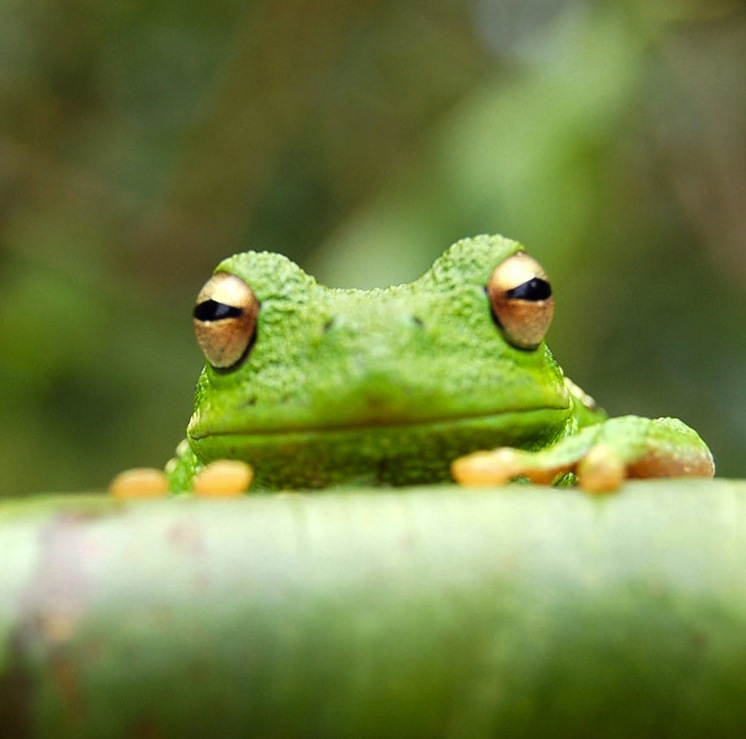
\includegraphics[width=0.7\linewidth]{frog}
\caption{An example image of a frog.}
\label{fig:view}
\end{figure}

\begin{table}[ht]
\centering
\begin{tabular}{l|r}
Item & Quantity \\\hline
Candles & 4 \\
Fork handles & ?  
\end{tabular}
\caption{\label{tab:widgets}An example table.}
\end{table}

\subsection*{Citations}

LaTeX formats citations and references automatically using the bibliography records in your .bib file, which you can edit via the project menu. Use the cite command for an inline citation, like \cite{lees2010theoretical}, and the citep command for a citation in parentheses \citep{lees2010theoretical}.

\subsection*{Mathematics}

\LaTeX{} is great at typesetting mathematics. Let $X_1, X_2, \ldots, X_n$ be a sequence of independent and identically distributed random variables with $\text{E}[X_i] = \mu$ and $\text{Var}[X_i] = \sigma^2 < \infty$, and let
$$S_n = \frac{X_1 + X_2 + \cdots + X_n}{n}
      = \frac{1}{n}\sum_{i}^{n} X_i$$
denote their mean. Then as $n$ approaches infinity, the random variables $\sqrt{n}(S_n - \mu)$ converge in distribution to a normal $\mathcal{N}(0, \sigma^2)$.

\subsection*{Lists}

You can make lists with automatic numbering \dots

\begin{enumerate}[noitemsep] 
\item Like this,
\item and like this.
\end{enumerate}
\dots or bullet points \dots
\begin{itemize}[noitemsep] 
\item Like this,
\item and like this.
\end{itemize}
\dots or with words and descriptions \dots
\begin{description}
\item[Word] Definition
\item[Concept] Explanation
\item[Idea] Text
\end{description}

\section*{Acknowledgments}

Additional information can be given in the template, such as to not include funder information in the acknowledgments section.

\bibliography{sample}

\end{document}